\documentclass[a4paper, 12pt]{article}

\newcommand\tab[1][.6cm]{\hspace*{#1}}
\usepackage[portuges]{babel}
\usepackage[utf8]{inputenc}
\usepackage{amsmath}
\usepackage{indentfirst}
\usepackage{graphicx}
\usepackage{multicol,lipsum}
\usepackage{blindtext}
\usepackage{verbatim}
\usepackage{textcomp}
\usepackage{hyperref}
\usepackage{float}
\usepackage{url}

\begin{document}
%\maketitle

\begin{titlepage}
	\begin{center}
	
	\begin{figure}[ht]
    \centering
    
\includegraphics[width=.44\textwidth]{LogoUFSJ.PNG}
    \label{fig:Capturar.PNG}
    \end{figure}

    	\Huge{Universidade Federal São João del Rei}\\
		\Large{Departamento de Ciência da Computação}\\ 

        \vspace{110pt}
        \textbf{\LARGE{
        \\
        \\
        \\
        Trabalho Prático 2: Relatório\\
        \vspace{0.5cm}
        \Large{Sistemas Operacionais}
        \\
        \\
        \\
        }}
        
		\title{{\large{Título}}}
		\vspace{2cm}
	\end{center}
	    
    \begin{flushleft}
		\begin{tabbing}
		\\
		\\
		\\	
		\large{Alunos: Paulo Victor Fernandes Sousa e Julio Cesar da Silva Rodrigues}\\
	    \\
		\large{Professor: Rafael Sachetto Oliveira}\\
	    \end{tabbing}
    \end{flushleft}
	\vspace{1cm}
	
	\begin{center}
		\vspace{\fill}
			Junho\\
		    2022
	\end{center}
\end{titlepage}

\tableofcontents
\newpage
\section{Introdução}

No contexto de sistemas operacionais, quando um computador necessita de uma quantidade superior de armazenamento à que a sua memória principal física é capaz de oferecer, ele utiliza de um mecanismo chamado substituição de páginas. Um sistema com suporte à memória virtual, apresenta nada mais do que páginas que são salvas e estão presentes no disco rígido e na memória principal dependendo de sua utilização. Isto fornece certa flexibilidade na gerência da memória como um todo, permitindo agilizar etapas de processamento de acordo a disposição das páginas entre memória principal e disco rígido, semelhante ao escalonamento de processos apresentado na primeira parte da disciplina.

Neste trabalho, é apresentado um simulador de memória virtual, uma tentativa de replicar as estruturas presentes em um mecanismo de gerência de memória, aplicando alguns algoritmos de substituição de página, com o objetivo de entender melhor como tais processos ocorrem, e como estes podem estar relacionados com aspectos de um sistema operacional.

\section{Estrutura Geral}

Toda a concepção da estrutura que compõe as páginas, assim como os algoritmos que às manipulam, incluindo os responsáveis por executar trocas de página, foram implementados em linguagem C. A implementação foi desenvolvida com o auxílio da ferramenta de controle de versionamento GitHub, e encontra-se disponível publicamente no repositório \url{https://github.com/juliorodrigues07/virtual_memory_sim}. Vale citar também que foram utilizados recursos da linguagem Python, mas apenas para utilização exclusiva na construção de gráficos, utilizando como métricas os resultados oriundos dos relatórios produzidos pela implementação em C do simulador de memória virtual, para realizar uma breve análise de desempenho que será discutida mais adiante neste trabalho.

Neste programa, dada uma entrada qualquer contendo a técnica de reposição à ser aplicada, a instância de teste (arquivo \emph{.log}), o tamanho das páginas e o total de memória disponível, o programa calcula o número máximo de páginas que a memória principal é capaz de armazenar simultaneamente. Em seguida, este pode criar uma nova página ou aplicar um algoritmo de substituição à medida que novos endereços são lidos, exibindo ao término da instância um breve relatório, contendo a configuração de entrada, número de páginas lidas e escritas, o número de faltas de páginas, e por fim, o número de páginas "sujas". Todas estas métricas são identificadas e coletadas ao longo do tempo de execução do programa.

A organização do código se apresenta de forma bastante simples. Além do \emph{header}, a implementação contém somente um \emph{script} de execução (main), e um \emph{script} contendo as funções essenciais e auxiliares para construção do simulador de memória virtual.

No \emph{header}, encontra-se a estrutura de dados que define cada página (\emph{Page}), e esta contém as seguintes variáveis:

\begin{itemize}
    \item \emph{id}: Responsável por armazenar o valor de identificação da página.
    \item \emph{modified}: \emph{Bit} que indica se a página foi modificada a cada interrupção de relógio.
    \item \emph{referenced}: \emph{Bit} que indica se a página foi referenciada a cada interrupção de relógio.
    \item \emph{usage}: Valor que será incrementado ou decrementado na aplicação do algoritmo \emph{LRU} para indicar a "idade" das páginas.
    \item \emph{next}: Ponteiro que aponta para o endereço da estrutura de dados da próxima página.
\end{itemize}

\subsection{Arquivo \emph{main.c}}

Presente neste arquivo está a função \emph{main}, que atua apenas como uma intermediadora na execução do programa. Nela é checada a corretude dos parâmetros informados pelo usuário, assim como a leitura dos arquivos \emph{.log} contendo endereços e modos de operação que serão então passados à outras funções responsáveis por lidar com estes dados.

É importante citar que nesta implementação, está presente uma interrupção de relógio que atua de acordo com a quantidade de endereços obtidos do arquivo. Definimos este valor aproximando o cálculo de 1\% do total de endereços contidos nas instâncias de teste, o que resultou em uma transição de \(1024\) operações, ou seja, a cada \(1024\) endereços lidos, todos os bits de referenciação das páginas presentes na memória principal são zerados.

Nesta mesma função, algumas métricas de execução já são coletadas (número de leituras, escritas...) à medida que certas funções são chamadas (\emph{page\_search} e \emph{write\_address}).

\subsection{Arquivo \emph{virtual\_mem\_sim.c}}

Neste \emph{script} se encontram as funções essenciais para o funcionamento do simulador. Nele estão presentes desde funções básicas auxiliares, como as de descarte de bits de endereço para identificação de páginas, até os algoritmos principais de paginação em si, que serão responsáveis por orquestrar as trocas de páginas, à medida que os endereços e modos de operação são lidos dos arquivos.

\subsubsection{Função \emph{add\_new\_page}}

Sabemos que, dada a intenção de acessar uma página, seja para leitura ou escrita, esta primeiro deve ser colocada na memória principal para garantir um acesso de maior velocidade em constraste com o tempo de acesso à um disco rígido. Esta função se encarrega justamente desta tarefa, criando novas páginas que não estejam na memória principal, inicializando seus atributos como \emph{id}, \emph{bit} de referência, utilização, e também o \emph{bit} de modificação, este que depende diretamente da operação que se deseja realizar (R ou W) junto com o endereço da página. 

Todas estas páginas criadas são organizadas em uma lista encadeada, e um contador é mantido para certificar que o número de páginas na memória principal não ultrapasse sua capacidade.

\subsubsection{Função \emph{fill\_info}}

Esta função poderá ser utilizada intensamente por quaisquer dos algoritmos de troca de página implementados. Nela são preenchidos os atributos da página à ser colocada na memória principal de forma similar à função \emph{add\_new\_page} citada anteriormente. A principal diferença encontrada aqui, é que a página selecionada para troca deixará de existir na memória principal, e caso esteja modificada, esta deve ser escrita novamente no disco. Em casos como este, são coletadas métricas sobre o número de páginas "sujas" que tiveram de ser escritas de volta no disco durante a execução do programa.

\subsubsection{Função \emph{lru}}

O funcionamento geral do algoritmo nesta implementação é bastante simples. Basicamente, a lista de páginas é percorrida, realizando uma busca pelo menor valor de utilização, ou seja, pela página mais velha ou a que está a mais tempo sem ser referenciada. Após encontrá-la, tal página é substituída utilizando a função \emph{fill\_info} descrita anteriormente.

A operação feita neste valor de utilização é apenas o deslocamento de um bit para a direita ou esquerda (dividir por 2 ou multiplicar por 2). A cada referenciação de uma determinada página, seu valor de utilização aumenta deslocando-se um bit para a esquerda, e a cada interrupção de relógio, este valor diminui deslocando-se um bit para a direita, operação que é aplicada sob todas as páginas presentes na memória principal.

\subsubsection{Função \emph{second\_chance}}

Talvez o algoritmo de troca de página mais simples presente nesta implementação, seu funcionamento também não é nada complexo. Desta vez, percorremos a lista analisando o bit de referenciação das páginas presentes na memória principal. O algoritmo percorre-a buscando por uma página que não foi referenciada na interrupção de relógio atual (cujo bit de referenciação é igual à zero). Durante este processo, se aplicável, é dada uma "segunda chance" para todas as páginas referenciadas que forem analisadas, movendo-as para o final da lista de páginas. Caso todas as páginas presentes na memória principal estejam referenciadas na interrupção de relógio atual, seleciona-se de forma automática a página presente na primeira posição da lista (similar ao algoritmo \emph{FIFO}).

\subsubsection{Função \emph{nru}}

Neste algoritmo, deixamos de operar sob valores \emph{booleanos} e passamos a dividir as páginas presentes na memória principal em classes. Assim como nos dois algoritmos descritos de forma breve anteriormente, também vamos percorrer a lista de páginas, mas desta vez analisando os bits de referenciação e modificação em conjunto. 

Dada a divisão em classes presente na própria concepção do algoritmo, são armazenadas no máximo quatro páginas (uma de cada classe) que serão analisadas em prioridade crescente (0 \(\rightarrow\) 1 \(\rightarrow\) 2 \(\rightarrow\) 3). A ação mais adequada sempre será a escolha de uma página da classe 0 (não referenciada e não modificada) se aplicável, enquanto a classe 3 se mostra como último recurso na execução da substituição. Resumindo, selecionamos a página que pertence à classe mais inferior possível em uma interrupção de relógio qualquer para substituição, que será realizada utilizando a função \emph{fill\_info} novamente. 

\subsubsection{Função \emph{page\_search}}

Esta também é uma das funções que apresentará uso mais intenso durante a execução do programa. Quaisquer endereços informados pelo arquivo de extensão \emph{.log} deverão primeiramente ser analisados se suas páginas correspondentes já estão presentes na memória principal, e por consequência, definir se a execução de um algoritmo de substituição de página será necessária. 

Novamente a lista é percorrida, e em caso do valor de identificação da página analisada estar presente na memória principal, os bits de referenciação e modificação são atualizados, assim como o valor de utilização conforme a operação realizada (escrita ou leitura). Em casos que páginas não são encontradas na memória principal, existem dois caminhos possíveis para lidar com tal situação. Uma nova página pode ser criada simplesmente utilizando a função \emph{add\_new\_page} caso exista espaço suficiente livre na memória, caso contrário, um algoritmo de substituição de página é executado, indicando uma falta de página que será coletada durante a execução.

\subsubsection{Função \emph{unreference\_pages}}

Esta se trata de uma função auxiliar simples, mas de grande importância na execução do programa. Sua principal tarefa é "marcar" todas as páginas presentes na memória principal como \textbf{não referenciadas} (alterando o bit de referenciação para zero e decrementando o valor de utilização) a cada interrupção de relógio.

\subsubsection{Função \emph{shift\_bits}}

Retirada da própria especificação do trabalho prático, esta função tem como tarefa única, o descarte de bits de endereço para obter a identificação da página. Seu funcionamento é flexível à variação do tamanho das páginas a cada execução independente.

\section{Problemas na Implementação}

À seguir, serão explanados de forma breve os principais problemas que encontramos durante o desenvolvimento deste trabalho.

\subsection{Tabelas de Página}

Neste trabalho, a principal funcionalidade que não está implemetada corretamente é a tabela de páginas. Devido a maior complexidade da construção de tal estrutura de forma reversa, não obtivemos sucesso na tentativa de implementá-la. Como mencionado anteriormente, a criação e manipulação das páginas é realizada utilizando uma estrutura de dados bastante simples, uma lista encadeada de páginas.

\subsection{Tempo de Execução e Otimização}

Embora as instâncias fornecidas para teste sejam de tamanho considerável, nossa implementação não se deparou com problemas no que diz respeito à longos períodos de execução. Acreditamos que isto aconteceu devido ao tamanho máximo de memória bastante discreto, especificado na proposta do trabalho prático. 

Em grande parte das funções implementadas percorremos a lista de páginas de forma íntegra, o que pode vir a se tornar um grande obstáculo em execuções cujo tamanho da memória é maior, possivelmente levando a tempos de execução excessivamente longos. Uma possível solução seria a proposta inicial da própria especificação, implementando uma tabela de páginas reversa, flexibilizando a manipulação das páginas.

\section{Execução}

Para compilar o programa, basta executar o seguinte comando via terminal:

\begin{center}
    \boxed{\textbf{\large{make}}}
\end{center}

Para a execução do programa é necessário informar o nome do executável, o nome do algoritmo, arquivo \emph{.log} de entrada, o tamanho das páginas e o tamanho da memória principal, como é exibido no exemplo abaixo:

\vspace{0.3cm}
\begin{center}
    \\\vspace{0.3cm}
    \boxed{\textbf{\large{./tp2virtual lru arquivo.log 32 128}}}
\end{center}
\vspace{0.3cm}

\section{Análise de Desempenho}

Como orientado na especificação deste trabalho, colocamos em teste o desempenho desta implementação utilizando as instâncias distintas fornecidas, além de variar o tamanho da memória e da página em baterias de testes separadas, utilizando como métricas o número de faltas de página e o número de páginas "sujas" totalizados ao decorrer da execução de cada algoritmo.

Com isto em mente, ao aplicarmos os testes, nos deparamos com alguns padrões que reforçam conceitos vistos na disciplina de Sistemas Operacionas, os quais se destacam, o crescimento do tamanho das páginas implicando no acréscimo da taxa de faltas de página, assim como a dimunuição do tamanho da memória obtendo o mesmo efeito. Em um contexto de tempo de execução, esses casos apresentaram melhores resultados, constrastando com o aumento no tempo de execução quando a valoração de tais parâmetros é invertida (menor tamanho de página e maior quantidade de memória).

Podemos citar de antemão como principal surpresa apresentada por estes testes, os resultados obtidos utilizando o arquivo de teste \emph{compressor.log} e mantendo fixo o tamanho da memória (Figura \ref{fig:exampleFig3}). Neste caso em específico, os algoritmos apresentaram pouquíssimas faltas de página e em nenhum momento apresentaram páginas sujas na execução. Mesmo quando o tamanho de página foi fixado, embora estes tenham apresentado faltas de página e páginas sujas inicialmente, suas taxas declinaram de forma excessivamente veloz, o que talvez possa indicar um viés quanto à distribuição dos dados do arquivo, ou até mesmo possíveis erros de implementação presentes nos algoritmos. Uma análise aprofundada desta instância seria de grande utilidade em conjunto com a aplicação destes testes.

Outra particularidade interessante observada foi o comportamento do algoritmo \emph{NRU}. Suas métricas em relação ao número de páginas sujas foram consistentemente menores do que os outros algoritmos.

Em relação à quantidade de faltas de páginas, os resultados obtidos foram bem difusos quando o tamanho da memória não é alterado, apresentando crescimentos e quedas lineares (exceto no caso do arquivo \emph{compressor.log}), ausentes de quaisquer padrões que possam ser observados à primeira vista. Tais informações podem ser observadas nos gráficos apresentados nas Figuras \ref{fig:exampleFig1}, \ref{fig:exampleFig2} e \ref{fig:exampleFig4}, que correspondem à métricas coletadas durante a execução dos algoritmos para os arquivos \emph{matriz.log}, \emph{compilador.log} e \emph{simulador.log}.

No restante dos casos, os relatórios apresentados pelos algoritmos foi ligeiramente parecido, apresentando crescimentos lineares para o número de faltas de página e páginas sujas à medida que o tamanho de página aumenta, e descréscimos exponenciais à medida que a capacidade da memória principal aumenta.

Os gráficos que sumarizam os dados observados nos testes realizados são exibidos nas Figuras \ref{fig:exampleFig1}, \ref{fig:exampleFig2}, \ref{fig:exampleFig3}, \ref{fig:exampleFig4}, \ref{fig:exampleFig5}, \ref{fig:exampleFig6}, \ref{fig:exampleFig7} e \ref{fig:exampleFig8}. Primeiramente são apresentados gráficos para tamanho de memória fixo, e na próxima subsseção, para tamanho de página fixo. São ilustrados os números absolutos de faltas de página e páginas sujas observados a cada arquivo analisado (\emph{matriz.log}, \emph{compilador.log}, \emph{compressor.log} e \emph{simulador.log}), respectivamente.

\subsection{Tamanho da Memória Fixo}

\begin{figure}[H]
    \centering
    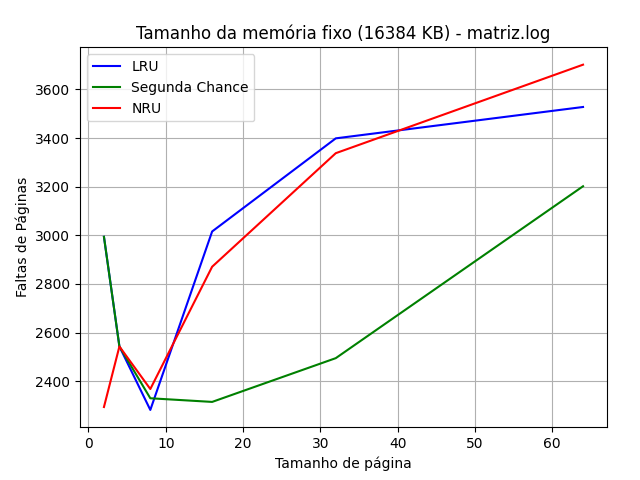
\includegraphics[width=0.9\textwidth]{fixed_mem/matriz/fault.png}
    \hspace{1.5cm}
    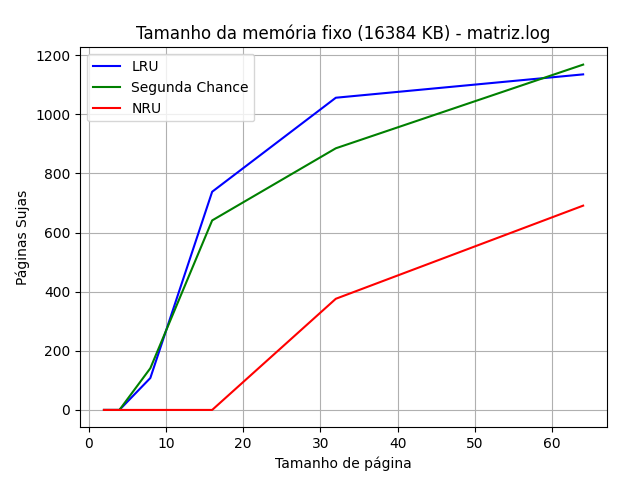
\includegraphics[width=0.9\textwidth]{fixed_mem/matriz/write.png}
    \caption{Comparativo de desempenho dos algoritmos (\emph{matriz.log})}
    \label{fig:exampleFig1}
\end{figure}

\begin{figure}[H]
    \centering
    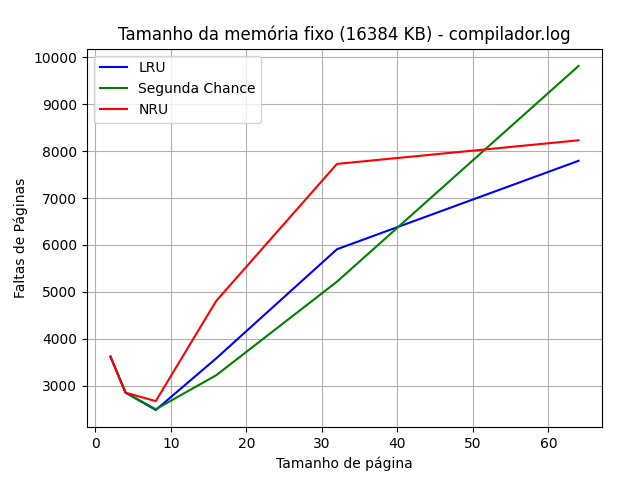
\includegraphics[width=0.92\textwidth]{fixed_mem/compilador/fault.png}
    \hspace{1.5cm}
    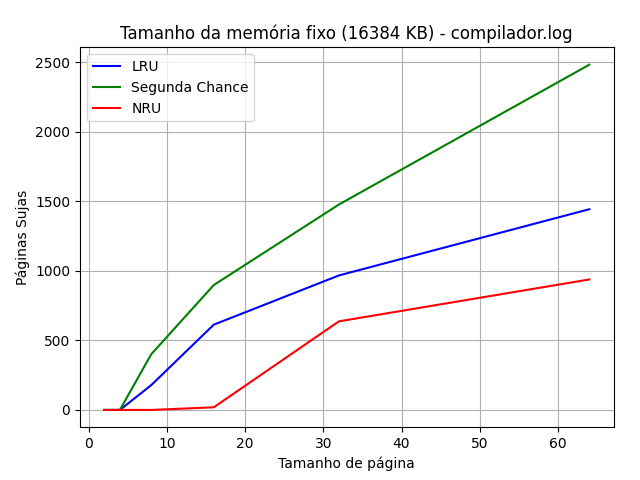
\includegraphics[width=0.92\textwidth]{fixed_mem/compilador/write.png}
    \caption{Comparativo de desempenho dos algoritmos (\emph{compilador.log})}
    \label{fig:exampleFig2}
\end{figure}

\begin{figure}[H]
    \centering
    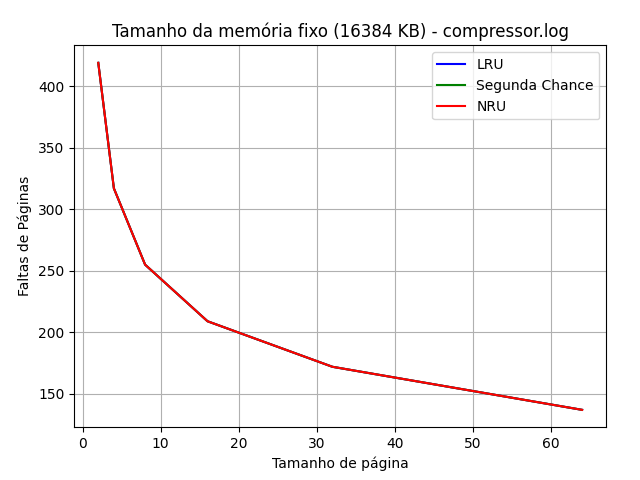
\includegraphics[width=0.92\textwidth]{fixed_mem/compressor/fault.png}
    \hspace{1.5cm}
    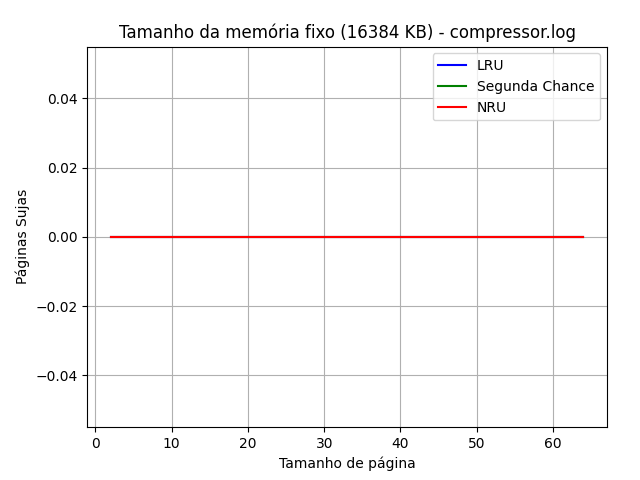
\includegraphics[width=0.92\textwidth]{fixed_mem/compressor/write.png}
    \caption{Comparativo de desempenho dos algoritmos (\emph{compressor.log})}
    \label{fig:exampleFig3}
\end{figure}

\begin{figure}[H]
    \centering
    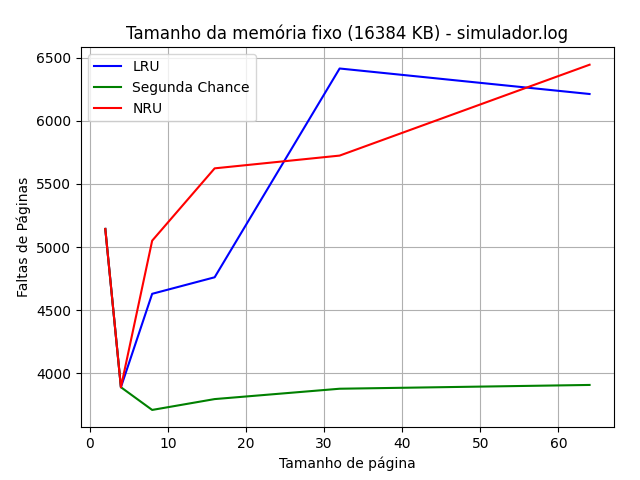
\includegraphics[width=0.92\textwidth]{fixed_mem/simulador/fault.png}
    \hspace{1.5cm}
    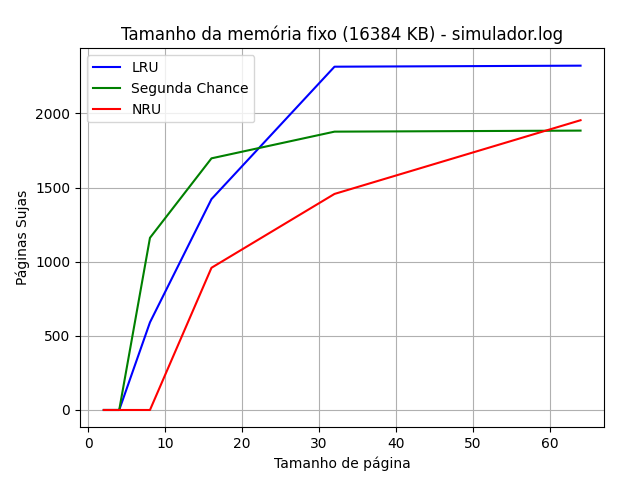
\includegraphics[width=0.92\textwidth]{fixed_mem/simulador/write.png}
    \caption{Comparativo de desempenho dos algoritmos (\emph{simulador.log})}
    \label{fig:exampleFig4}
\end{figure}

\subsection{Tamanho de Página Fixo}

\begin{figure}[H]
    \centering
    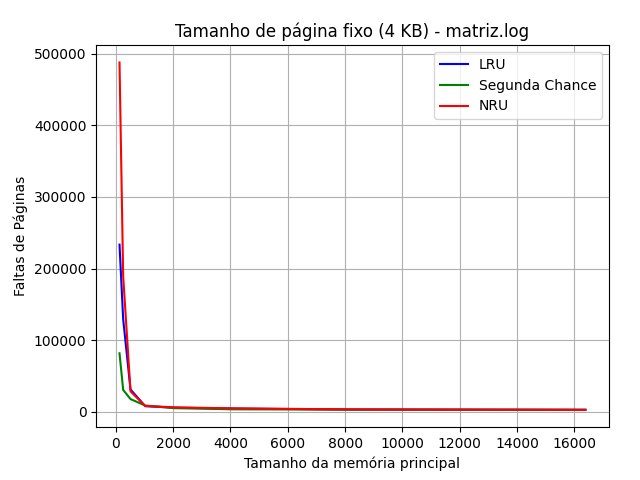
\includegraphics[width=0.9\textwidth]{fixed_pag/matriz/fault.png}
    \hspace{1.5cm}
    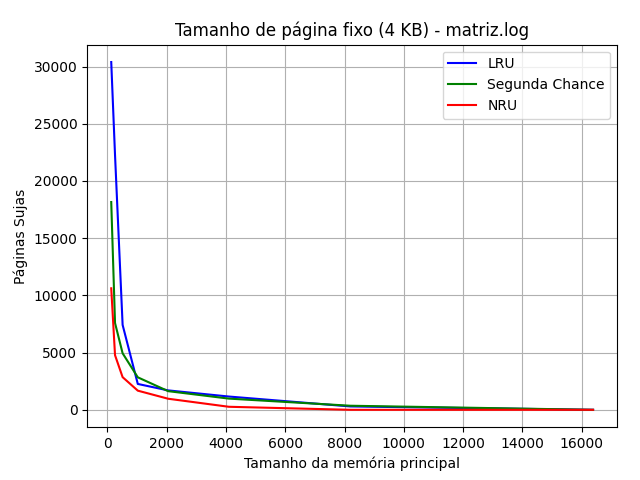
\includegraphics[width=0.9\textwidth]{fixed_pag/matriz/write.png}
    \caption{Comparativo de desempenho dos algoritmos (\emph{matriz.log})}
    \label{fig:exampleFig5}
\end{figure}

\begin{figure}[H]
    \centering
    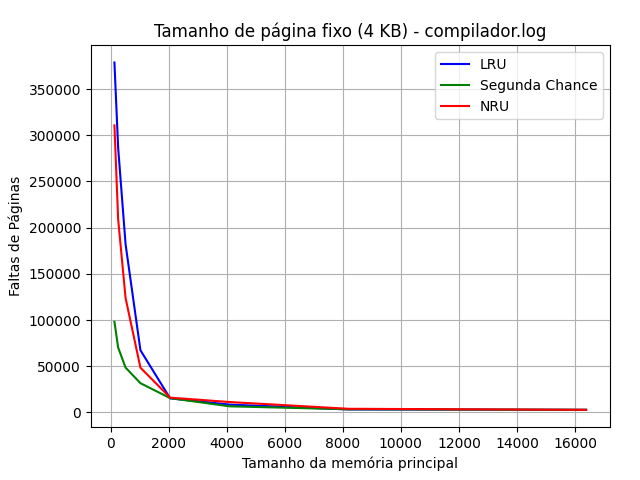
\includegraphics[width=0.92\textwidth]{fixed_pag/compilador/fault.png}
    \hspace{1.5cm}
    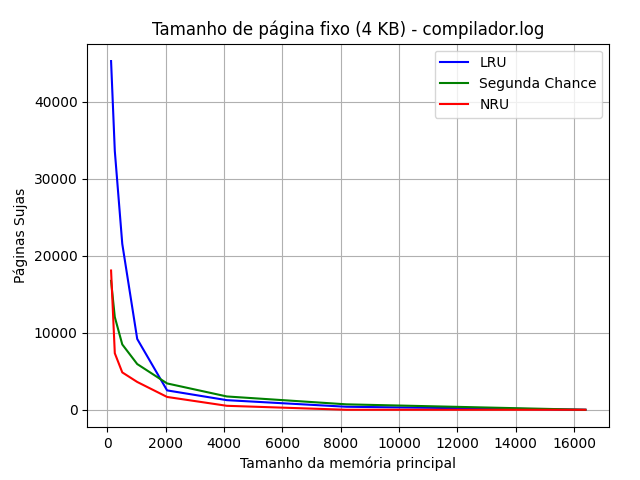
\includegraphics[width=0.92\textwidth]{fixed_pag/compilador/write.png}
    \caption{Comparativo de desempenho dos algoritmos (\emph{compilador.log})}
    \label{fig:exampleFig6}
\end{figure}

\begin{figure}[H]
    \centering
    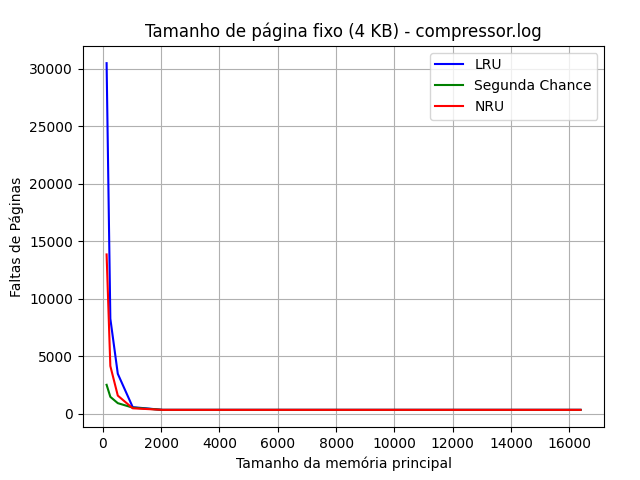
\includegraphics[width=0.92\textwidth]{fixed_pag/compressor/fault.png}
    \hspace{1.5cm}
    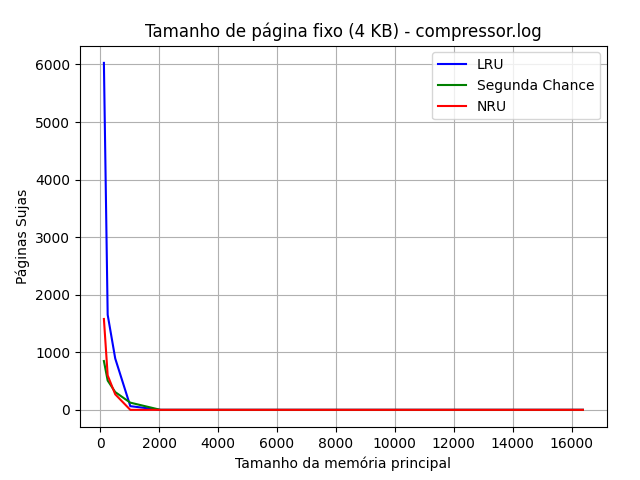
\includegraphics[width=0.92\textwidth]{fixed_pag/compressor/write.png}
    \caption{Comparativo de desempenho dos algoritmos (\emph{compressor.log})}
    \label{fig:exampleFig7}
\end{figure}

\begin{figure}[H]
    \centering
    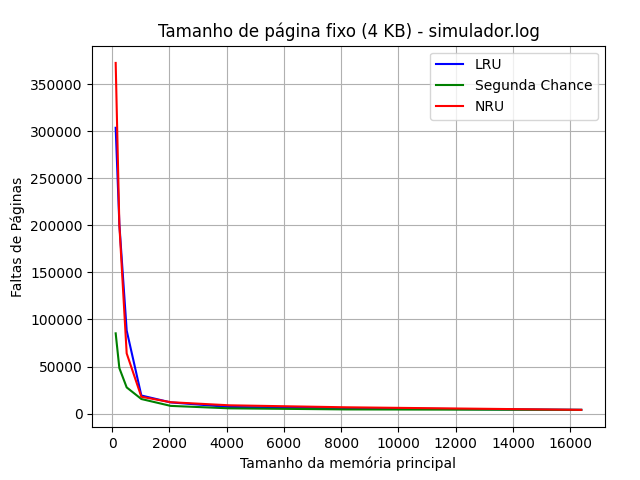
\includegraphics[width=0.92\textwidth]{fixed_pag/simulador/fault.png}
    \hspace{1.5cm}
    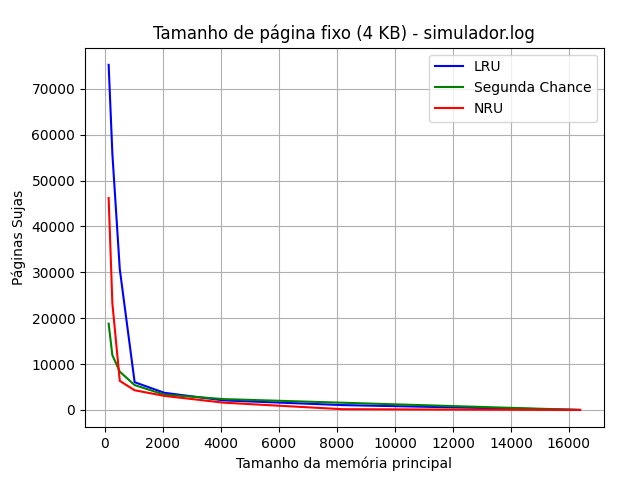
\includegraphics[width=0.92\textwidth]{fixed_pag/simulador/write.png}
    \caption{Comparativo de desempenho dos algoritmos (\emph{simulador.log})}
    \label{fig:exampleFig8}
\end{figure}

\section{Considerações Finais}

Neste trabalho, foi construído um simulador de memória virtual com o objetivo de compreender de forma mais clara, como ocorre o gerenciamento da memória virtual feita pelo componente \emph{MMU}. Nele podemos observar de forma nítida, a complexidade por trás do controle de paginação essencial que é requisitado de forma constante em sistemas com memória reais. 

Além disso, foi analisado a forma como o tamanho das páginas e o tipo de algoritmo utilizado na paginação respondem às distintas distribuições das páginas. Isto mostra a complexidade de se encontrar a melhor forma de se manipular páginas e gerenciar mecanismos de memória virtual. Por isto, consideramos que a parte mais complexa do desenvolvimento deste trabalho, em que enfrentamos as maiores dificuldades foi na tentativa da implementação da tabela de paginação.

Por fim, acreditamos que foi possível compreender um pouco mais a fundo as nuanças por trás da  manipulação de páginas e gerência da memória virtual, tarefas bastantes complexas que exigem um software eficiente, simples, e principalmente, robusto, pouco ou nada suscetível à erros fatais.

\section*{Referências}
\begin{itemize}
    \item Gerenciamento de Memória Virtual - Algoritmos de Paginação: \url{http://wiki.icmc.usp.br/images/d/dc/Aula12.pdf}
    \item Not Recently Used (NRU) page replacement algorithm: \url{https://www.geeksforgeeks.org/not-recently-used-nru-page-replacement-algorithm/}
\end{itemize}

\end{document}
